\documentclass{article}
\usepackage{vmargin}
\setpapersize{USletter} %Tamaño del papel
\setmargins{2.54cm} % Maren Izquierda
{2.54cm} %Margen superior
{16.52cm} %Ancho del texto
{22.82cm} %Altura del texto
{0.2cm} %Altura de los encabezados
{1cm} %Espacio entre los textos
{1cm} %Altura del pie de pagina
{1cm} %Espacio entre el texto y el pie de pagina
\usepackage[utf8]{inputenc}
\usepackage[spanish]{babel}
\usepackage{graphicx}
\graphicspath{ {images/} }
\usepackage{cite}


\begin{document}
	
	\begin{titlepage}
		\begin{center}
			\vspace*{1cm}
			
			\Huge{\textbf{Nociones de la memoria del computador}}
			
			\vspace{7cm}
			
			\Large{\textbf{Autor:}\\Juan Alejandro Gualteros Fonseca}
			
			\vfill
			
			\vspace{0.5cm}
			
			\Large
			Despartamento de Ingeniería Electrónica y Telecomunicaciones\\
			Universidad de Antioquia\\
			Medellín\\
			Septiembre - 2020
			
		\end{center}
	\end{titlepage}
	
	\newpage
	
	\tableofcontents
	
	\newpage
	
	\section{Introducción}\label{intro}
	Dentro de la computación hay muchos temas propios, que son de gran interés no solo por ser fundamentales para diseñar nuestra sociedad actual, sino también porque representan grandes avances, que hace apenas unas décadas eran impensables y que hoy hacen parte de la cotidianidad.\\
	Entre esos está la memoria, como componente fundamental para el funcionamiento de un ordenador, de cualquier nivel. Ahora es muy fácil definir memoria como la capacidad de almacenar y procesar información, pero esta descripción no nos dice como hace un dispositivo eléctrico para guardar algo intangible en esencia, es un avance muy merecido de nuestra época y que merece un concienzudo análisis, algo que este informe tratara de hacer. 
	
	\newpage
	
	\section{Defina que es la memoria del computador} \label{defina}
	Cuando hablamos de memoria en un contexto general, nos referimos a la capacidad de retener información, y luego poder acceder a ella en el momento más indicado, en el ámbito informático la memoria es el dispositivo que retiene y almacena los datos informáticos durante un periodo de tiempo, la memoria otorga una función fundamental en la computación moderna, el almacenamiento de la información y del conocimiento de una manera accesible y rápida.\cite{memoria}
	\\\\
	En su descripción moderna la memoria, suele referirse a una forma de almacenamiento en estado sólido, donde se guardan los datos que se usan en el momento presente, una mejor descripción seria memoria RAM (Random Access Memory), memoria de acceso aleatorio o Memoria Volátil\cite{monografia}, se llama así porque el procesador accede a la información que está en la memoria en cualquier punto sin tener que acceder a la información anterior o posterior. Es la memoria que se actualiza constantemente mientras el ordenador está en uso y que pierde sus datos mientras el ordenador se apaga.
	\\\\
	El propósito del almacenamiento es guardar datos que el computador no esté usando. Dicho almacenamiento tiene tres ventajas sobre la “Memoria”(\ref{rom}):
	
	\begin{enumerate}
		
		\item Hay espacio en almacenamiento que en “Memoria”
		\item El almacenamiento retiene su contenido cuando se apaga el computador
		\item Es más barato que la “Memoria”
		
	\end{enumerate}

	 Lo cual en la computación actual viene siento represando por un tiempo especial de memoria que es la Memoria no volátil, o memoria ROM (read-only memory), lo que permite la lectura de la información y no su escritura independientemente de la presencia o no de energía.
	 \begin{figure}[h]
	 	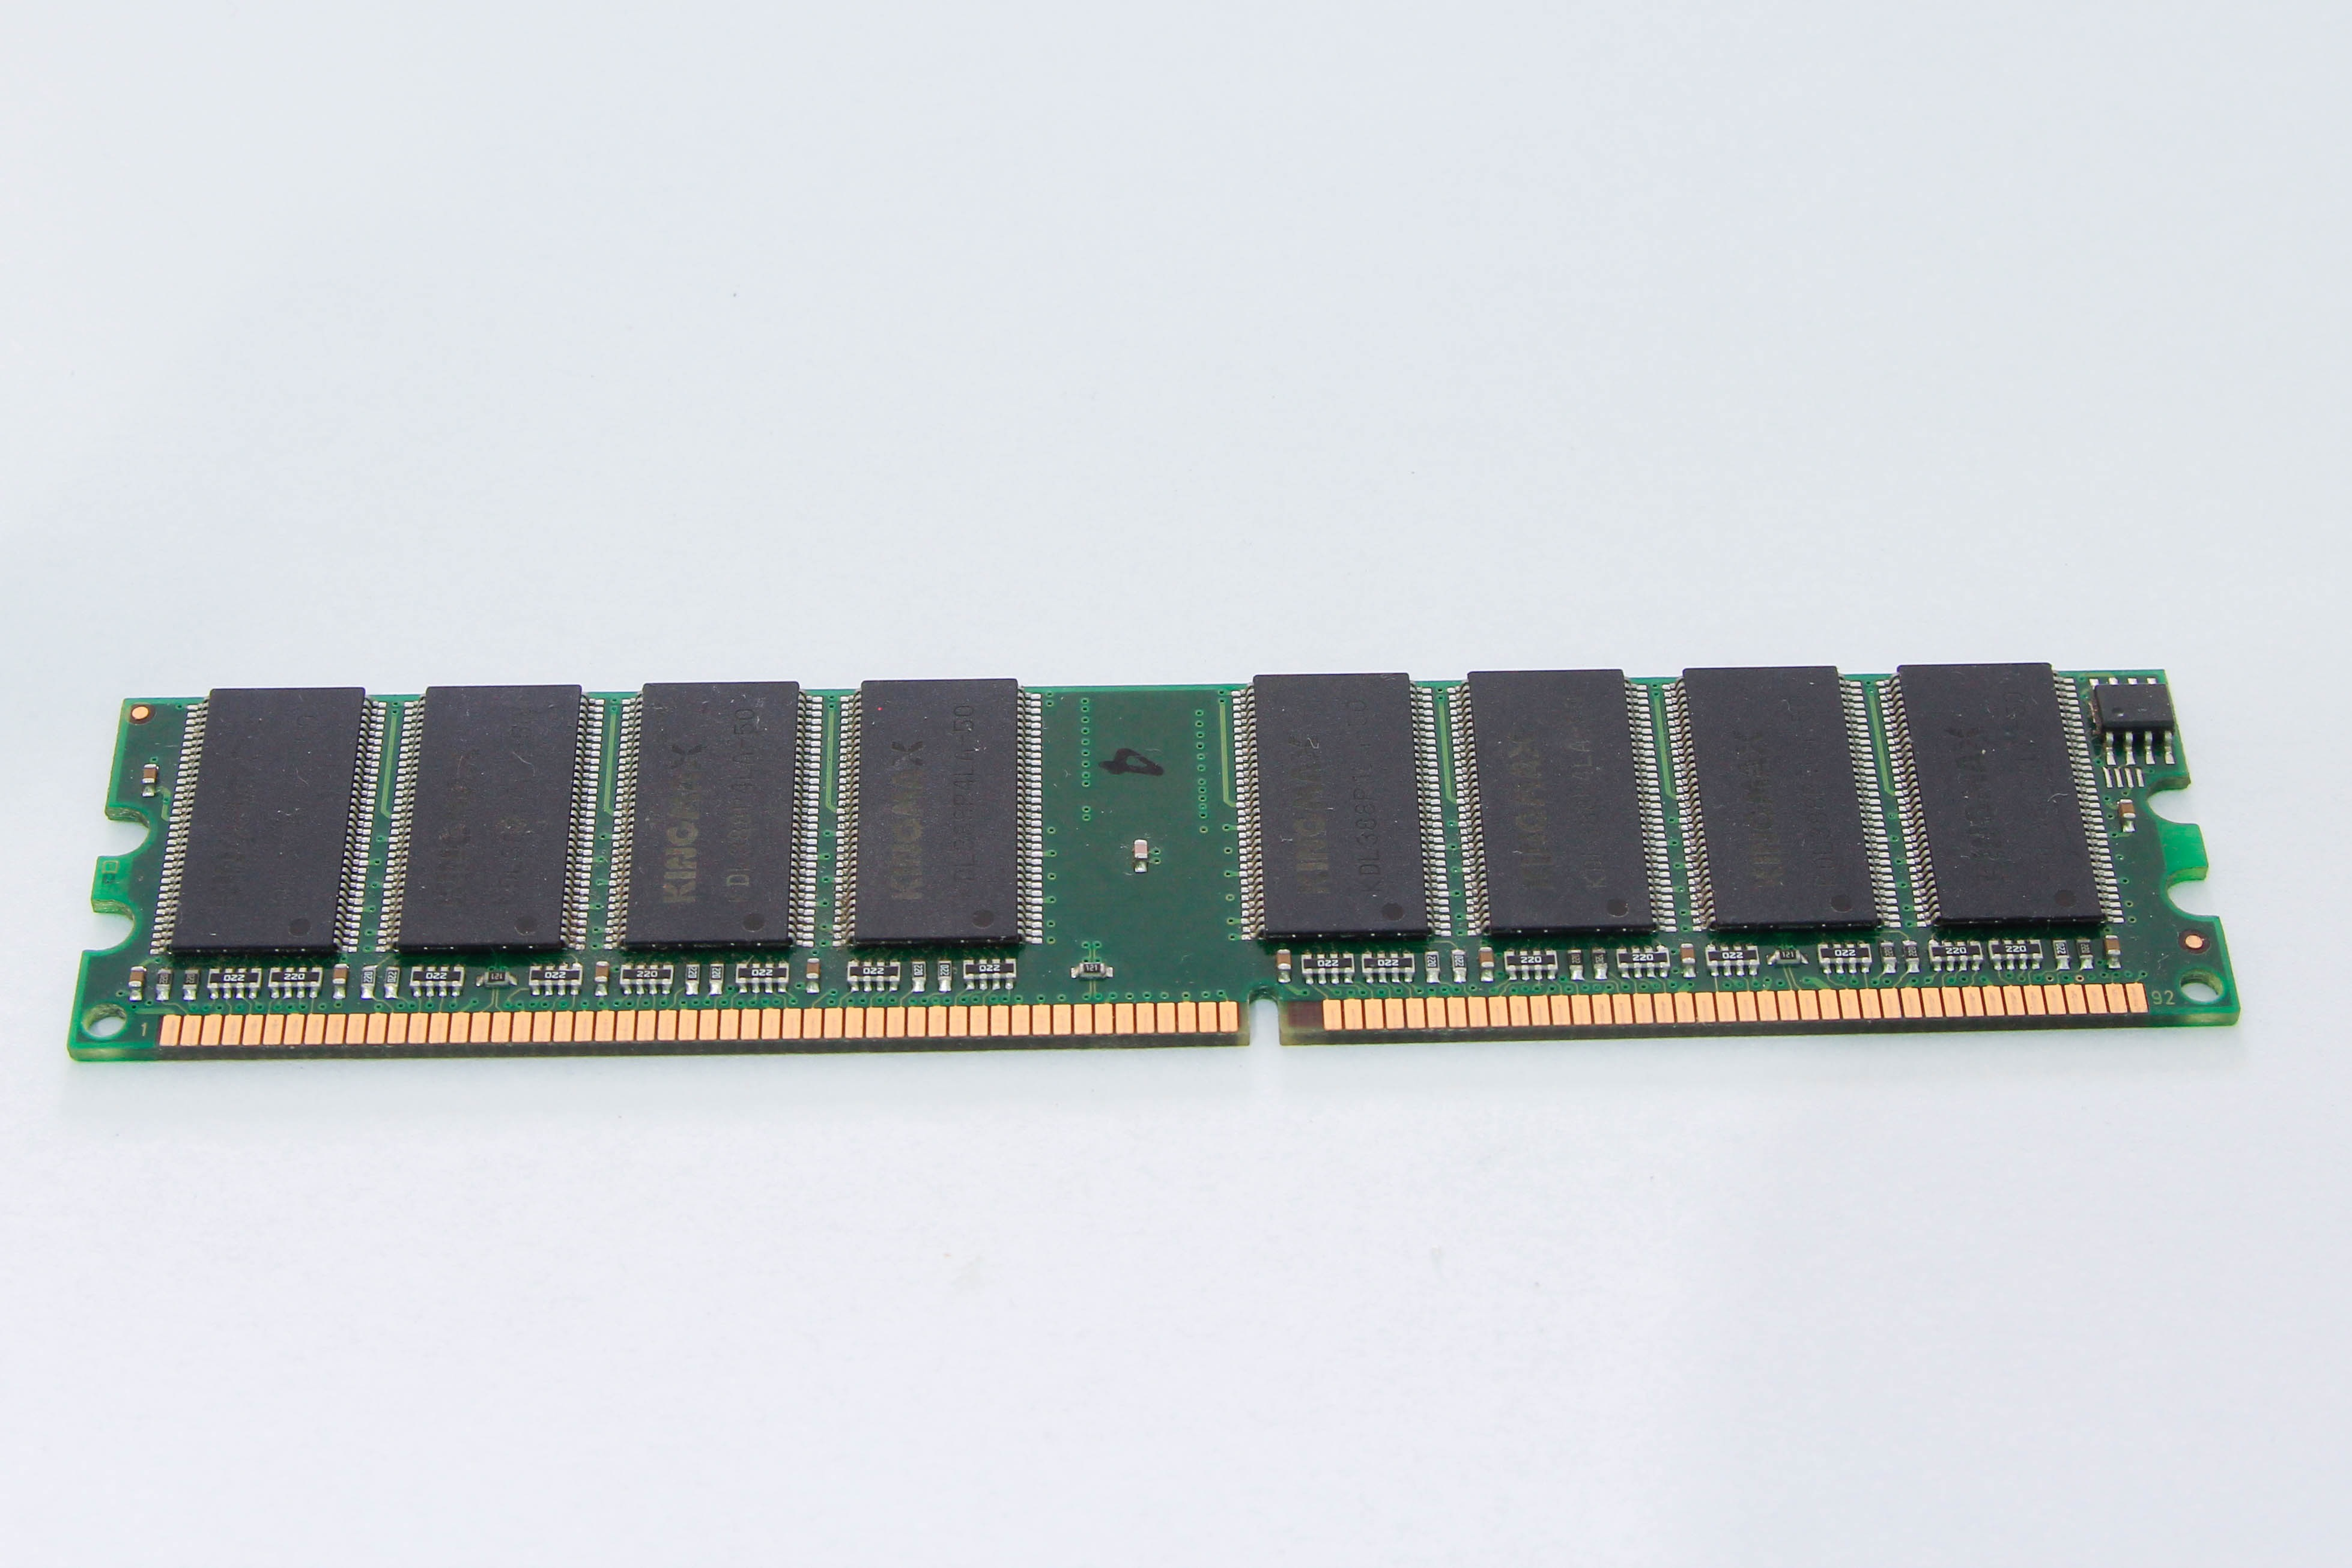
\includegraphics[width=4cm]{ram.jpg}
	 	\centering
	 	\caption{Memoria RAM}
	 	\label{ram}
	 \end{figure}
 
	 Para hacer una correcta analogía, un trabajador tiene que entregar los informes contables de una compañía, para ello tiene una Gaveta o caja para almacenarlo y una mesa con un libro contable y distintos formularios para su trabajo, mientras el trabajador se encuentra analizando la información que posee y transcribiéndola correctamente dentro de los formularios y el libro,(función que dentro del computador realiza el procesador), esta queda almacenada en distintos documentos que se pueden tomar como paquetes de información, cuando la jornada laboral del trabajador termina este guarda dichos paquetes en la Gaveta y termina su turno laboral, en el entorno digital, la mesa el libro y los formularios representan la memoria volátil, la cual solo está en uso mientras se requiera pero cuando el trabajador se va deja de usarcé, y la Gaveta la Memoria no volátil que cuando el trabajar termina almacena la información a la espera que esta vuelva a ser requerida.
	 
	\newpage
	
	\section{Menciona dos tipos de memoria que conoce y haga una pequeña descripción de cada una} \label{menciona}
	En un computador hay varios tipos de memoria, ordenados en jerarquías de velocidad y
capacidad, en este caso se muestran unas de una gran relevancia:\cite{youbioit}
	
	\begin{enumerate}
		
		\item Memoria Cache L1, L2 y L3
		\item Memoria RAM
		\item Memoria RAM
		\item Disco Duro
		
	\end{enumerate}
	
	\subsection{Memoria Cache L1, L2, L3}
	Actualmente hay microprocesadores de demasiado rápido que funciona a miles de millones de  ciclos por segundo, por lo cual requiere un dispositivo de almacenamiento temporal, de alta velocidad que pueda seguirle el ritmo, de lo contrario la velocidad se desperdiciaría a esperar que la información llegue, pero ese tipo de memorias y a esa velocidades resultan ser demasiados costosas, por lo que se dio como solución utilizar la memoria Cache que es la memoria más veloz en pequeñas cantidades secundadas, y la memoria RAM en grandes cantidades de almacenamiento falsh (\ref{ram}), ya que cada vez que se toma un paquete de datos del procesador se toma una copia por la memoria Cache.\cite{cache}
	\\\\
	Su función como memoria intermedia, que guarda los datos para que soluciones futuras por lo que esos datos se pueden atender con mayor rapidez, pueden ser el resultado de un cálculo anterior,\cite{cache} o como derivados de almacenamientos de un proceso, es una memoria intermedia su función es la velocidad. Algo que en el análisis de datos y a la velocidad de los procesadores, es muy necesario.
	
	\subsection{Memoria Virtual}
	Es una porción del disco duro, en tercer grado de jerarquía en la velocidad del disco duro, que está dedicada exclusivamente a “sostener”, temporalmente los pedazos de los programas, y datos en ejecución que se utilizan menos, o que ocupan un espacio innecesario en algún momento determinado y es preferible colocarlos en una zona de reserva, donde siempre estarán listos para ser utilizados cuando se les requiera, pero no ocuparán innecesariamente espacio en la memoria.
	
	\subsection{Disco Duro}
	EL disco duro es de un procesamiento comparativo más lento que las opciones anteriores ya que guardar la información aquí, procede a tardar más con la intención de conservar la información después de que le ordenador no tenga energía, por lo que se conoce como memoria no volátil, lo cual nos permite guardar información importante para su uso cuando iniciemos el equipo, mientras tanto el guardar la información de forma nativa, demora algo más de tiempo que las opciones anteriores, aunque y también depende mucho el tipo de disco duro si es de estado sólido (SSD) o unidad de disco fuerte (HDD).
	
	\begin{figure}[h]
		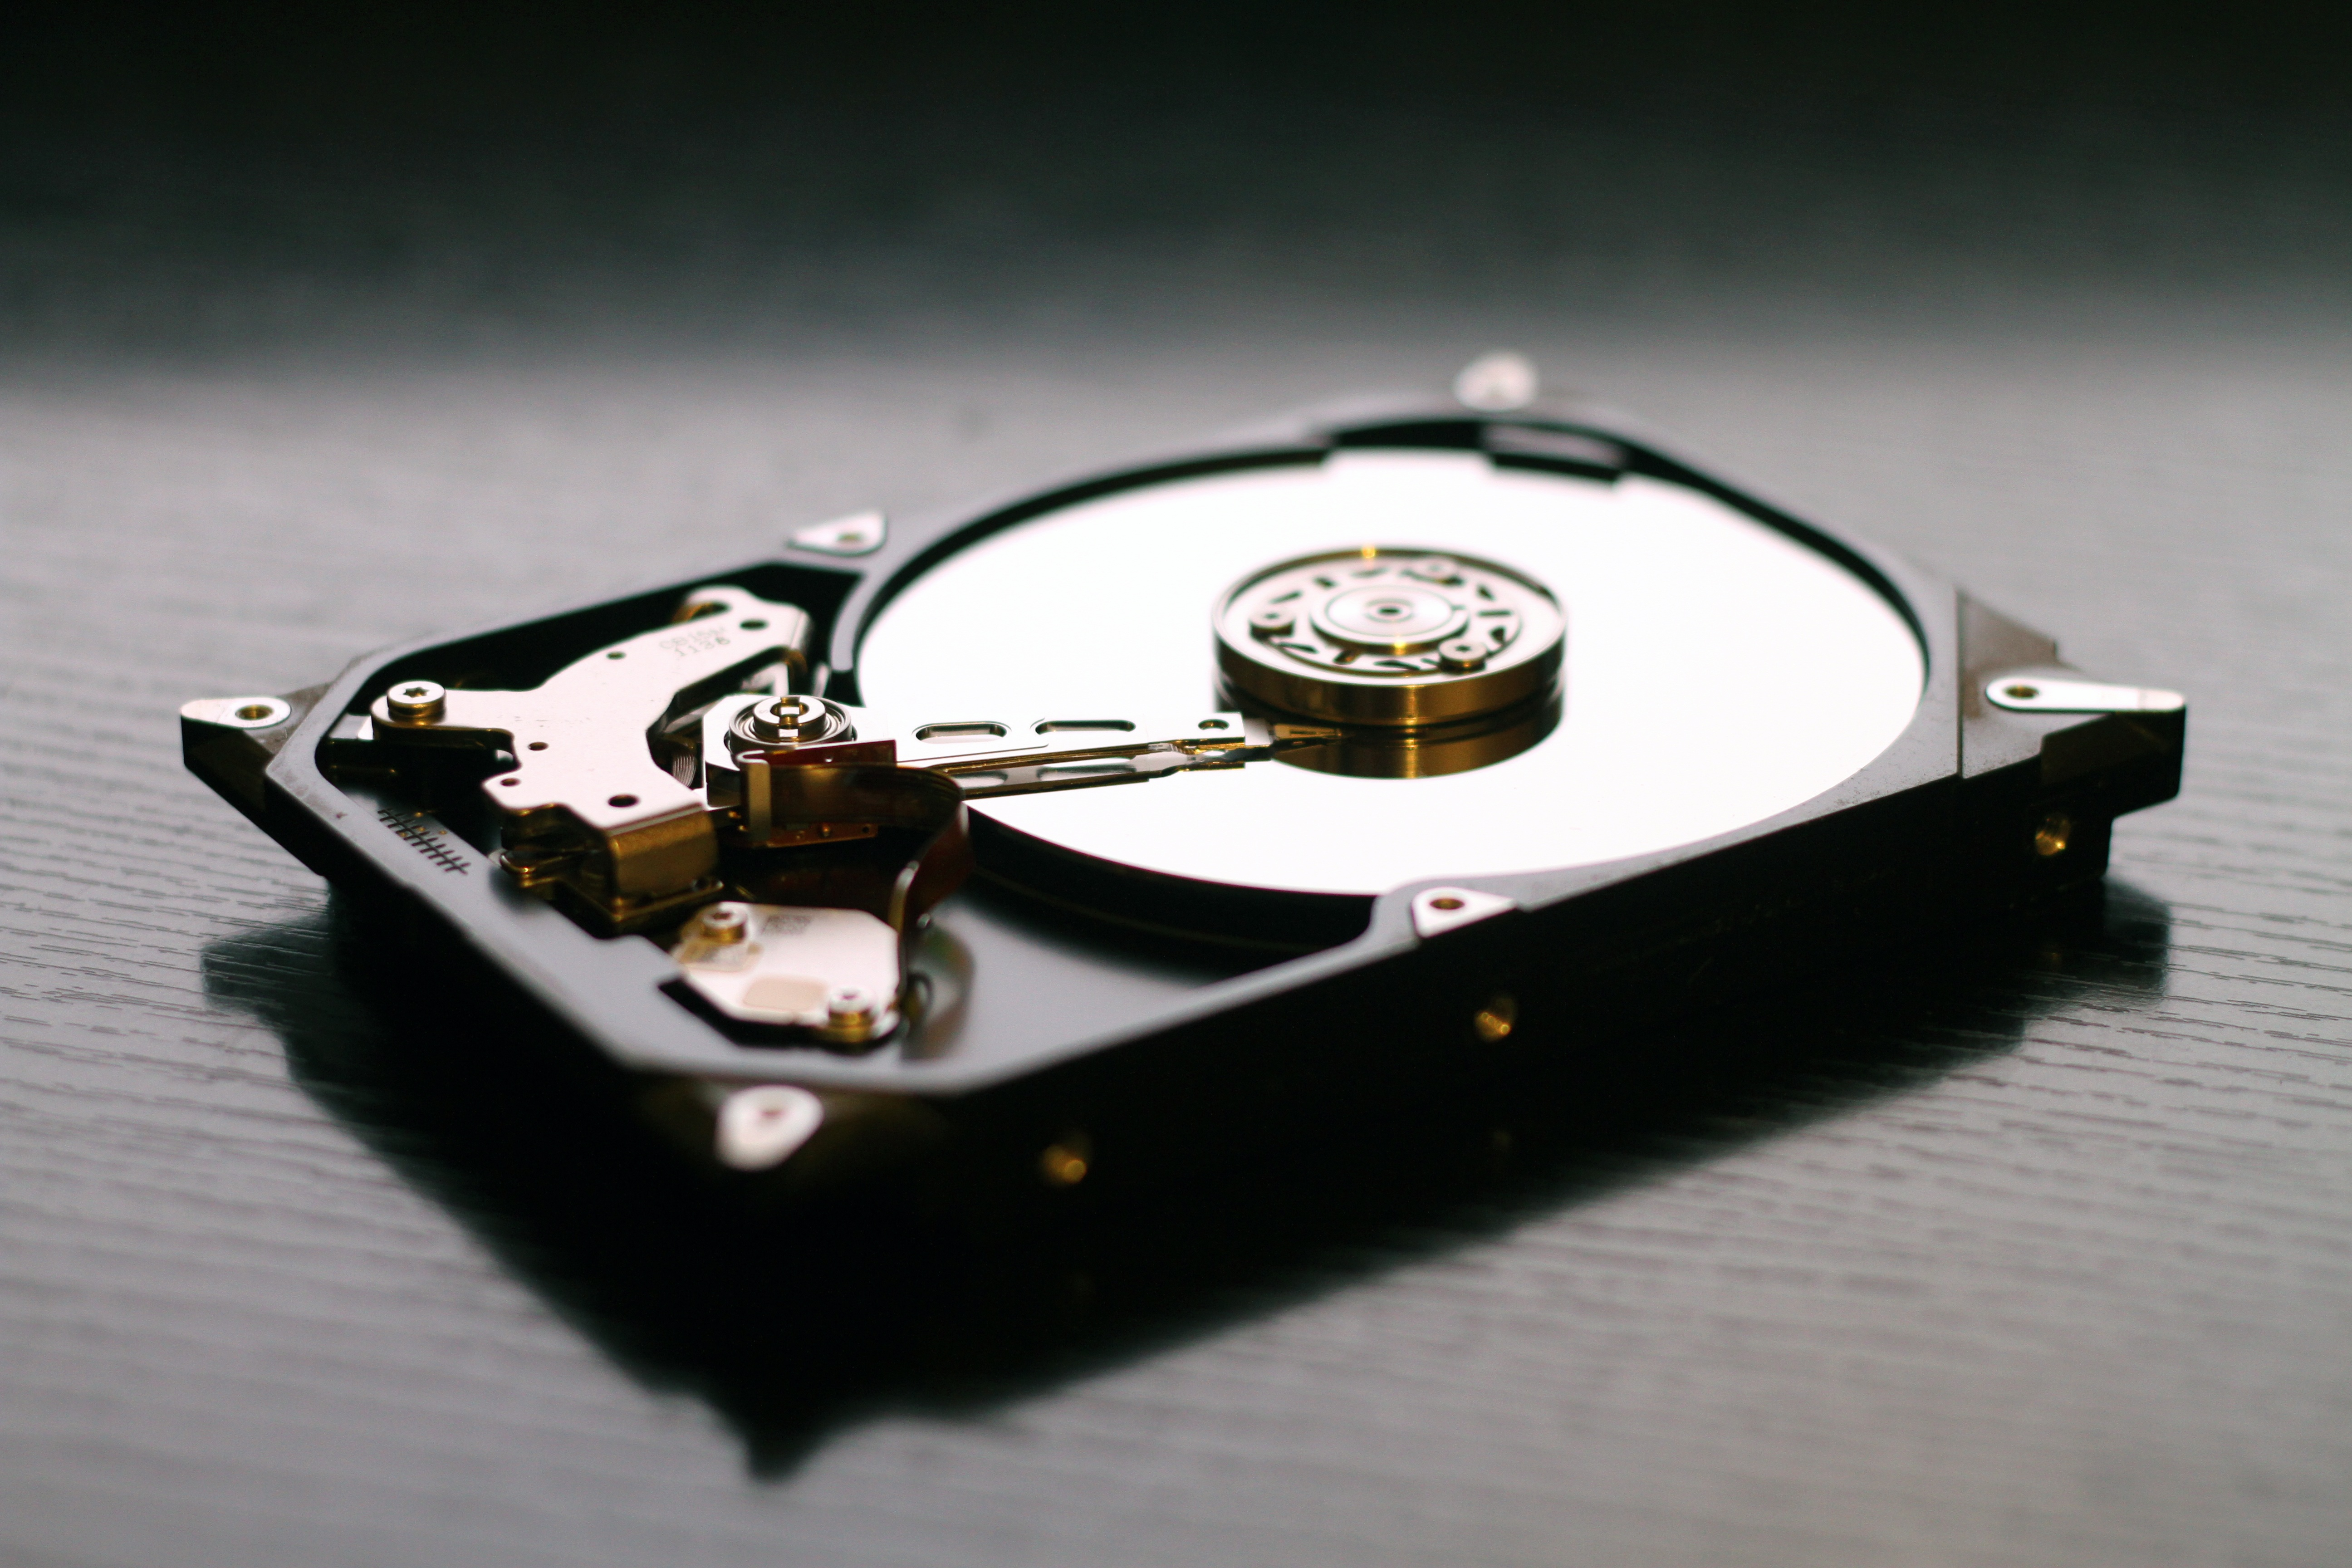
\includegraphics[width=4cm]{rom.jpg}
		\centering
		\caption{Disco Duro}
		\label{rom}
	\end{figure}
	
	\section{Describa la manera como se gestiona la memoria\\de un computador} \label{describa}
	Cuando nos referimos a gestionar, hablamos de la manera como el computador organiza y administra los datos de memoria del computador, y un muy buen ejemplo es la memoria RAM, dicha memoria está dividida en celdas de memoria, donde se almacena cada uno de los bits o pulsos eléctricos, (que representa 1 y 0), de las cuales se puede acceder directa e indistintamente, de sus posición y dirección.\cite{monografias}
	\\\\
	El procesador es el centro de trabajo del computador, dicho procesador tiene microcontroladores que para la fecha trabajan a velocidades incalculables hace unas décadas, la grandes velocidades actuales han permitido mejorar mucho procesos pero también conllevan una gran reto por igual, ya que la memoria no puede correr a la misma velocidad y ergo tener costos de trabajo y manutención accesibles, así que una buena manera de manejar le trabajo paralelo al procesador sin conocer los eventos que vaya a realizar el ordenador, \cite{youbioit} es trabajar con memoras de distinta velocidad y capacidad de almacenamiento para distintos propósito, de ahí nace la idea de usar la memoria caché como intermediario y preliminar, a la memoria RAM por lo que después permite al manejar la información de manera volátil, según el uso que se requiera dentro del computador, ya que su trabajo en mayor o menor medida requiere un gran esfuerzo por parte de la máquina, para después almacenar los datos necesarios en la memoria no volátil, pasando según el traslado de información en la memoria virtual, ya que es un vínculo directo entre la memoria RAM, y el disco duro o la memoria ROM, por lo que si se quiere guardar dicha información en líneas de comandos de bits, para almacenadas en el disco duro, y guardarlas a posteriori el computador este apagado.

	
	\section{¿Que hace que una memoria sea más rápida que otra?\\¿Porque eso es importante?} \label{que}
	Su diseño, cada memoria tiene una función distinta, y cada tipo de memoria debe estar diseñada de forma distinta para cumplir en especial con su función,\cite{youbioit} el formato de celdas es muy aplicable en memorias volátiles, ya que necesitan que el paso de la información sea rápida y conciso según los pulsos eléctricos, dicho trabajo a diferencia de las otras memorias hace que requieran una arquitectura más específica para los temas de análisis de datos, parecido al procesador, distinto del disco duro cuyo único fin es almacenar la información y que a lo largo del tiempo ha cambiado mucho su diseño y la tecnología que usa para guardar dicha información.
	\\\\
	Es importante ya que las función de cada parte de la memoria tiene que cumplir específicamente con su rango de trabajo, por eso es que en las memorias volátiles prima la velocidad que en la cantidad del almacenamiento y a mayor velocidad menor cantidad de almacenamiento procesal algo que le permite poder ejecutarse de manera más competa dentro del ordenador, el disco duro por poseer diferente arquitectura y cuya función es mantener la fidelidad de los datos se espera que sea más lento ya que se demora más tiempo es procesar y guardar la información.
	
	\newpage
	
	\section{Conclusión} \label{conclusion}
	En respuesta a todo lo analizado anteriormente, queda más que claro la importancia de la memoria, y de cada uno de sus tipos individuales para el funcionamiento de un ordenador, un equipo de cómputo que se puede tratar del más complejo hasta la placa más simple ya que siempre habrá una necesidad intrínseca de analizar y guardar información dentro cada proceso que se realice con equipos similares.
	\\\\
	El entender de manera más general como es el funcionamiento de estos equipos nos permite poder diseñar programas más especializados para y adaptados para un buen uso de la memoria entre otros recursos del computador, saber que con una programación correcta y un diseño eficaz se pueden mejorar muchos procesos ya se cuenta con una tecnología actual capaz de realizar infinidad de cosas que hace no mucho eran un sueño, el desarrollo de trabajos con respecto a estos conocimientos sera de gran ayuda en el futuro.
	
	\newpage
	
		
	\bibliographystyle{IEEEtran}
	Hola
	\bibliography{references}


\end{document}